\vspace*{-5mm}
\mysection{Architectural Design}

\mysubsection{Overview}
In this chapter we will analyze the proposed architecture and components of the Travlendar+ system.\par
The proposed architecture has three tiers :
\begin{itemize}
	\setlength{\leftskip}{0.5cm}
	\item \emph{Presentation Tier : }represented by Browser and Mobile App. It's how the system shows himself to the user.
	\item \emph{Presentation Tier : }represented by Web Server, which contains javascript and html code in order to create dynamic pages, and Application Server, which contains all the system's logic.
	\item \emph{Database Tier : }represented by DB Server, that contains and manages persistent data in an efficient way.
\end{itemize}
\begin{figure}[H]
	\centering
	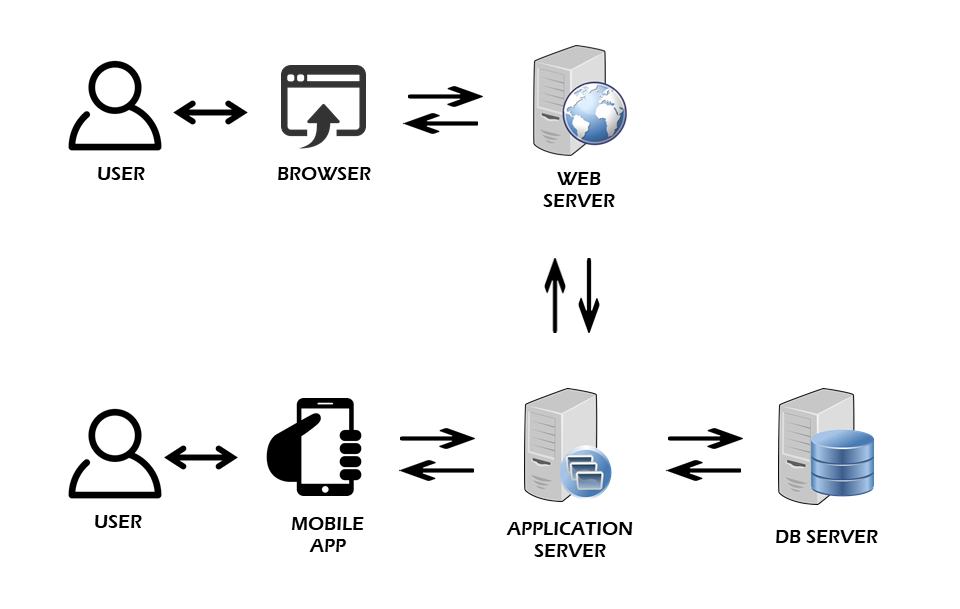
\includegraphics[scale=0.4]{Images/Architecture/Proposed_Architecture}
	\caption{Proposed Architecture}
\end{figure}

\mysubsection{High Level Components and Their Interactions}

TEXT HERE

\begin{figure}[H]
	\centering
	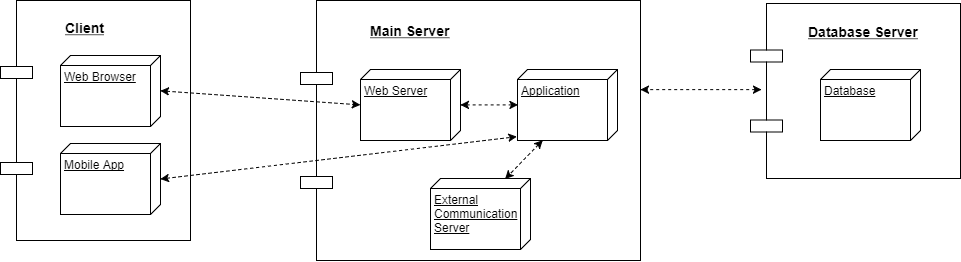
\includegraphics[scale=0.4]{Images/Architecture/Components_High_Level}
	\caption{Components High Level}
\end{figure}

\mysubsection{Component View}

TEXT HERE

\begin{figure}[H]
	\centering
	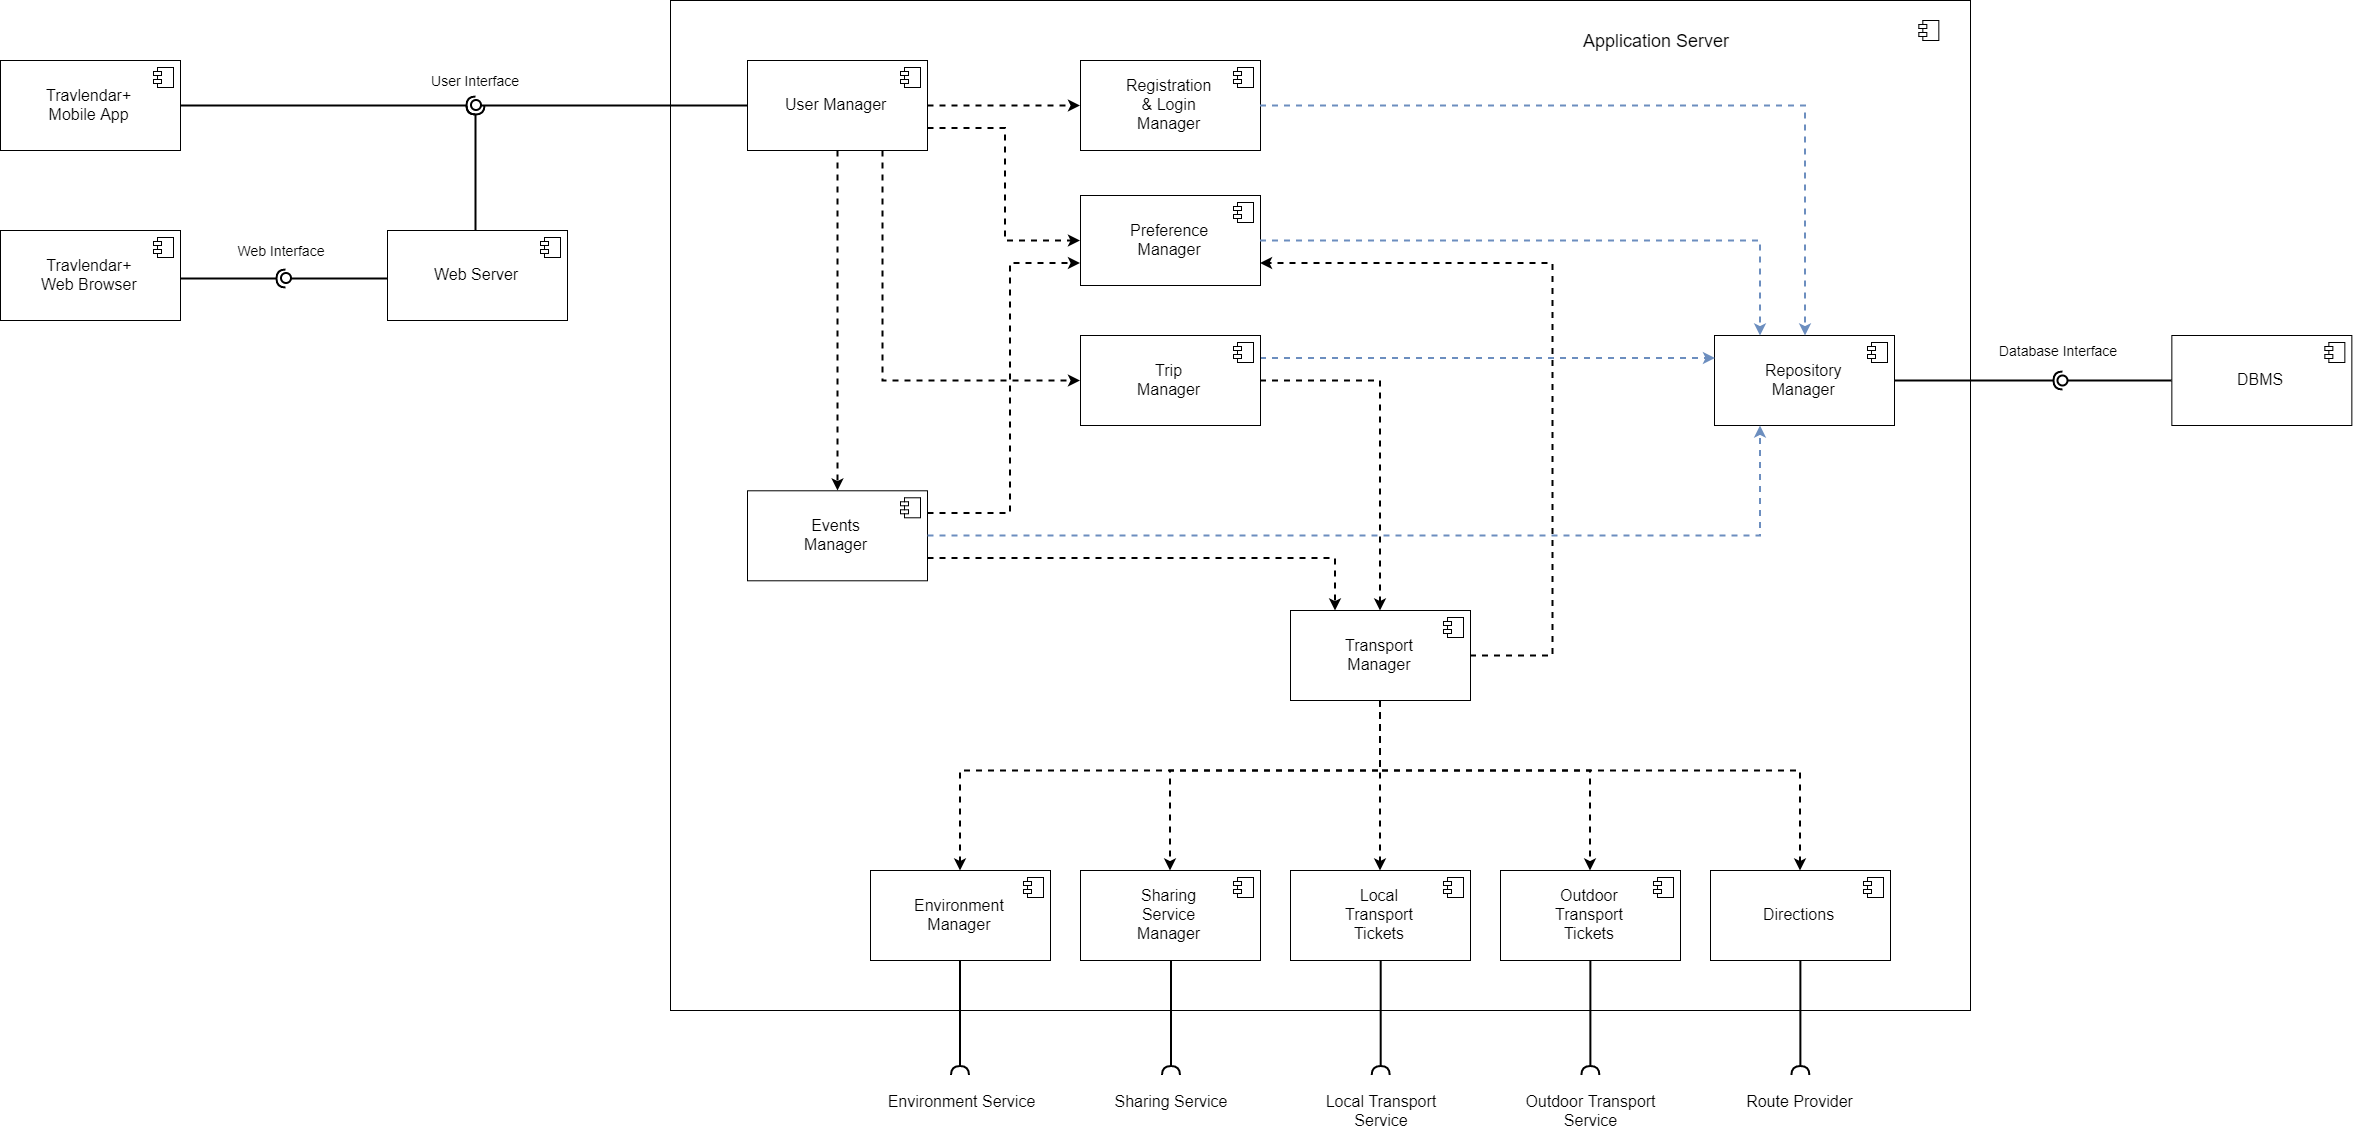
\includegraphics[scale=0.2]{Images/Architecture/Components_View}
	\caption{Component View}
\end{figure}

\mysubsection{Deployment View}

TEXT HERE

\mysubsection{Runtime View}

TEXT HERE

\mysubsection{Selected Architectural Styles and Patterns}

TEXT HERE

\mysubsection{Other Design Decisions}

TEXT HERE